
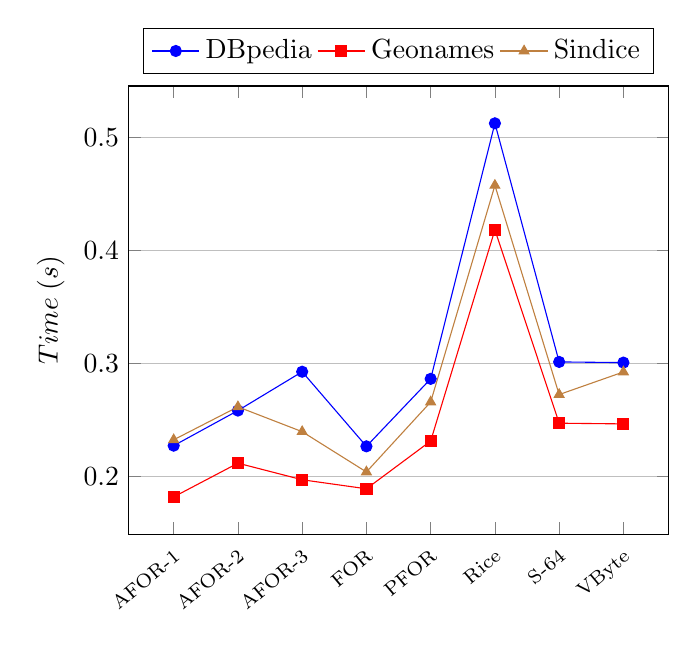
\begin{tikzpicture}
\begin{axis}[
ylabel=$Time \; (s)$,
x tick label style={font=\scriptsize, rotate=40, anchor=north east},
xtick={1,...,8},
xticklabels={AFOR-1, AFOR-2, AFOR-3, FOR, PFOR, Rice, S-64, VByte},
legend style={at={(0.5,1.13)}, anchor=north, legend columns=-1},
%ybar,
ymajorgrids=true,
%bar width=5pt,
]

\addplot[blue,mark=*]
coordinates {(1, 0.2271) (2, 0.2582) (3, 0.2926) (4, 0.2265) (5, 0.2863) (6, 0.5127) (7, 0.3013) (8, 0.3007)};
\addplot[red,mark=square*]
coordinates {(1, 0.1817) (2, 0.2116) (3, 0.1969) (4, 0.1889) (5, 0.2312) (6, 0.4184) (7, 0.2470) (8, 0.2464)};
\addplot[brown,mark=triangle*]
coordinates {(1, 0.2323) (2, 0.2615) (3, 0.2395) (4, 0.2038) (5, 0.2658) (6, 0.4577) (7, 0.2724) (8, 0.2924)};

\legend{DBpedia, Geonames, Sindice}

\end{axis}
\end{tikzpicture}%
